%%% Local Variables:
%%% coding: utf-8
%%% mode: latex
%%% TeX-engine: xetex
%%% End:
\documentclass[12pt,a4paper, ngerman, oneside]{scrartcl}
\usepackage[ngerman]{babel}
\usepackage[utf8]{inputenc}
\usepackage{ucs}
\usepackage{amsmath}
\usepackage{amsfonts}
\usepackage{amssymb}
\usepackage{graphics}
\usepackage{paralist}
\usepackage{floatflt} % grafiken die vom text umflossen werden
\usepackage{gensymb} % degree symbol
\usepackage{array} % grafiken in tabellen
\usepackage[linkcolor=black]{hyperref}
\usepackage{listings} \lstset{numbers=left, numberstyle=\tiny, numbersep=5pt} \lstset{language=Java}
%% Grafiken
\usepackage[pdftex]{graphicx}
\usepackage{epsfig}
\hypersetup{%
  colorlinks=true,
}

\newcommand\blfootnote[1]{%
  \begingroup
  \renewcommand\thefootnote{}\footnote{#1}%
  \addtocounter{footnote}{-1}%
  \endgroup
}
\hypersetup{
  pdfborder = {0 0 0},
  urlbordercolor = {0 0 0},
  colorlinks = true,
  linkcolor = black,
  citecolor = black,
  filecolor = black,
  urlcolor  = black
}
% Variablen
% siehe http://tex.stackexchange.com/a/290504 option 4
\def\Tiles/{8}
\def\Rundenlimit/{20}
\def\PointsPerTile/{7}
\def\PointsPerPassenger/{7}
\def\FieldsPerTile/{20}
\def\Passagiere/{5}

\newcommand{\fieldGraphic}[2]{%
\begin{floatingfigure}[#1]{0.15\textwidth}%
  \centering
  \includegraphics[width=0.15\textwidth]{bilder/#2}%
\end{floatingfigure}%
}

\sloppy
\hyphenpenalty=100000

\usepackage{fontspec}
\setromanfont{Merriweather}
\setsansfont{Lato}
\renewcommand{\normalsize}{\fontsize{12}{18}\selectfont}


\titlehead{
  \centering
\includegraphics[width=3.5cm]{bilder/logo.png}
}
\subject{Software-Challenge 2017}
\title{Spielregeln}
\subtitle{Mississippi Queen}
\date{Stand: \today}


\begin{document}
\maketitle
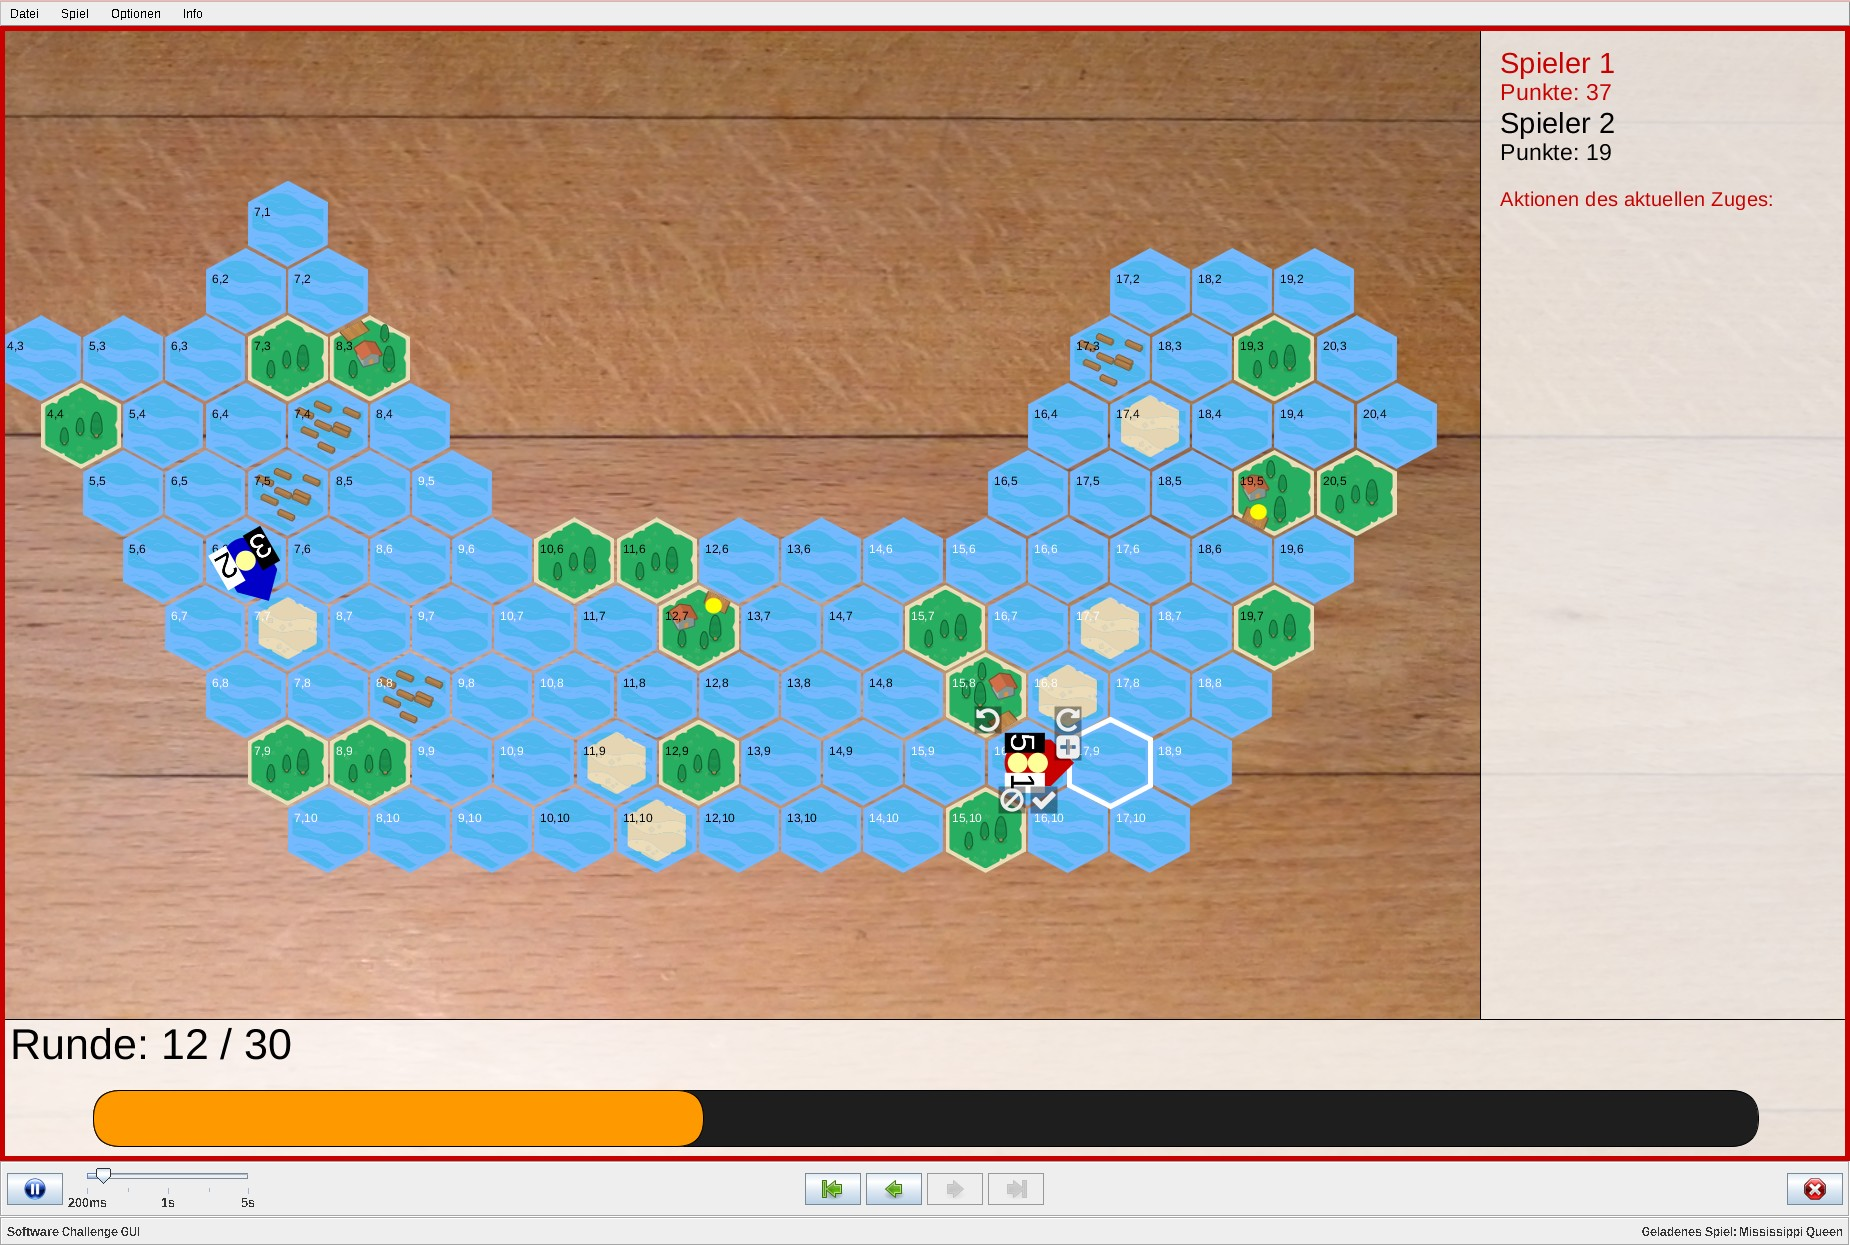
\includegraphics[width=\textwidth]{bilder/spielfeld-gross.jpg}
%\begin{figure}[!htbp]
%  \centering
%  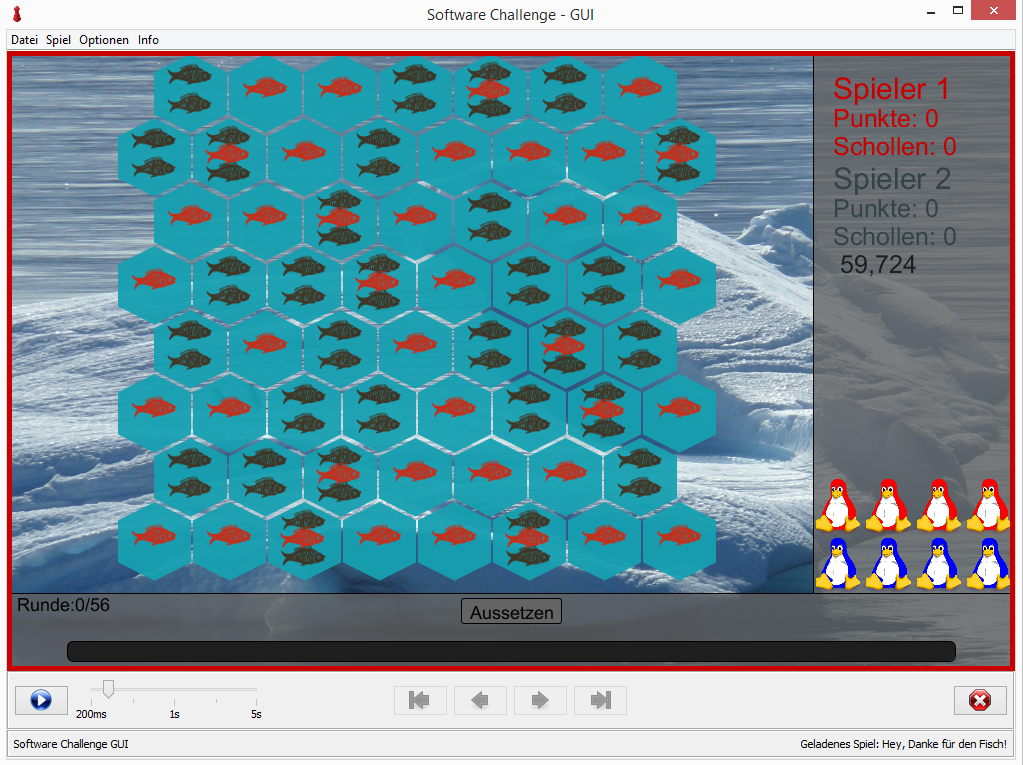
\includegraphics[width=\linewidth]{bilder/gui.png}
%\end{figure}
\vspace*{\fill}
\thispagestyle{empty}

\newpage
\tableofcontents
\thispagestyle{empty}
\newpage
\setcounter{page}{1}

\section{Einleitung}

In dieser Anleitung werden die Elemente und Regeln des Spiels Mississippi Queen
der Software-Challenge 2017 erläutert. Bei Mississippi Queen versuchen zwei
Spieler, durch abwechselndes Setzen von Raddampfern schnellstmöglich einen Fluss
bis zum Ziel entlangzufahren und dabei unterwegs zwei Passagiere mitzunehmen.
Der Spieler, dessen Dampfer das Ziel mit zwei Passagieren an Bord zuerst
erreicht, gewinnt das Spiel.


\section{Das Spielbrett}

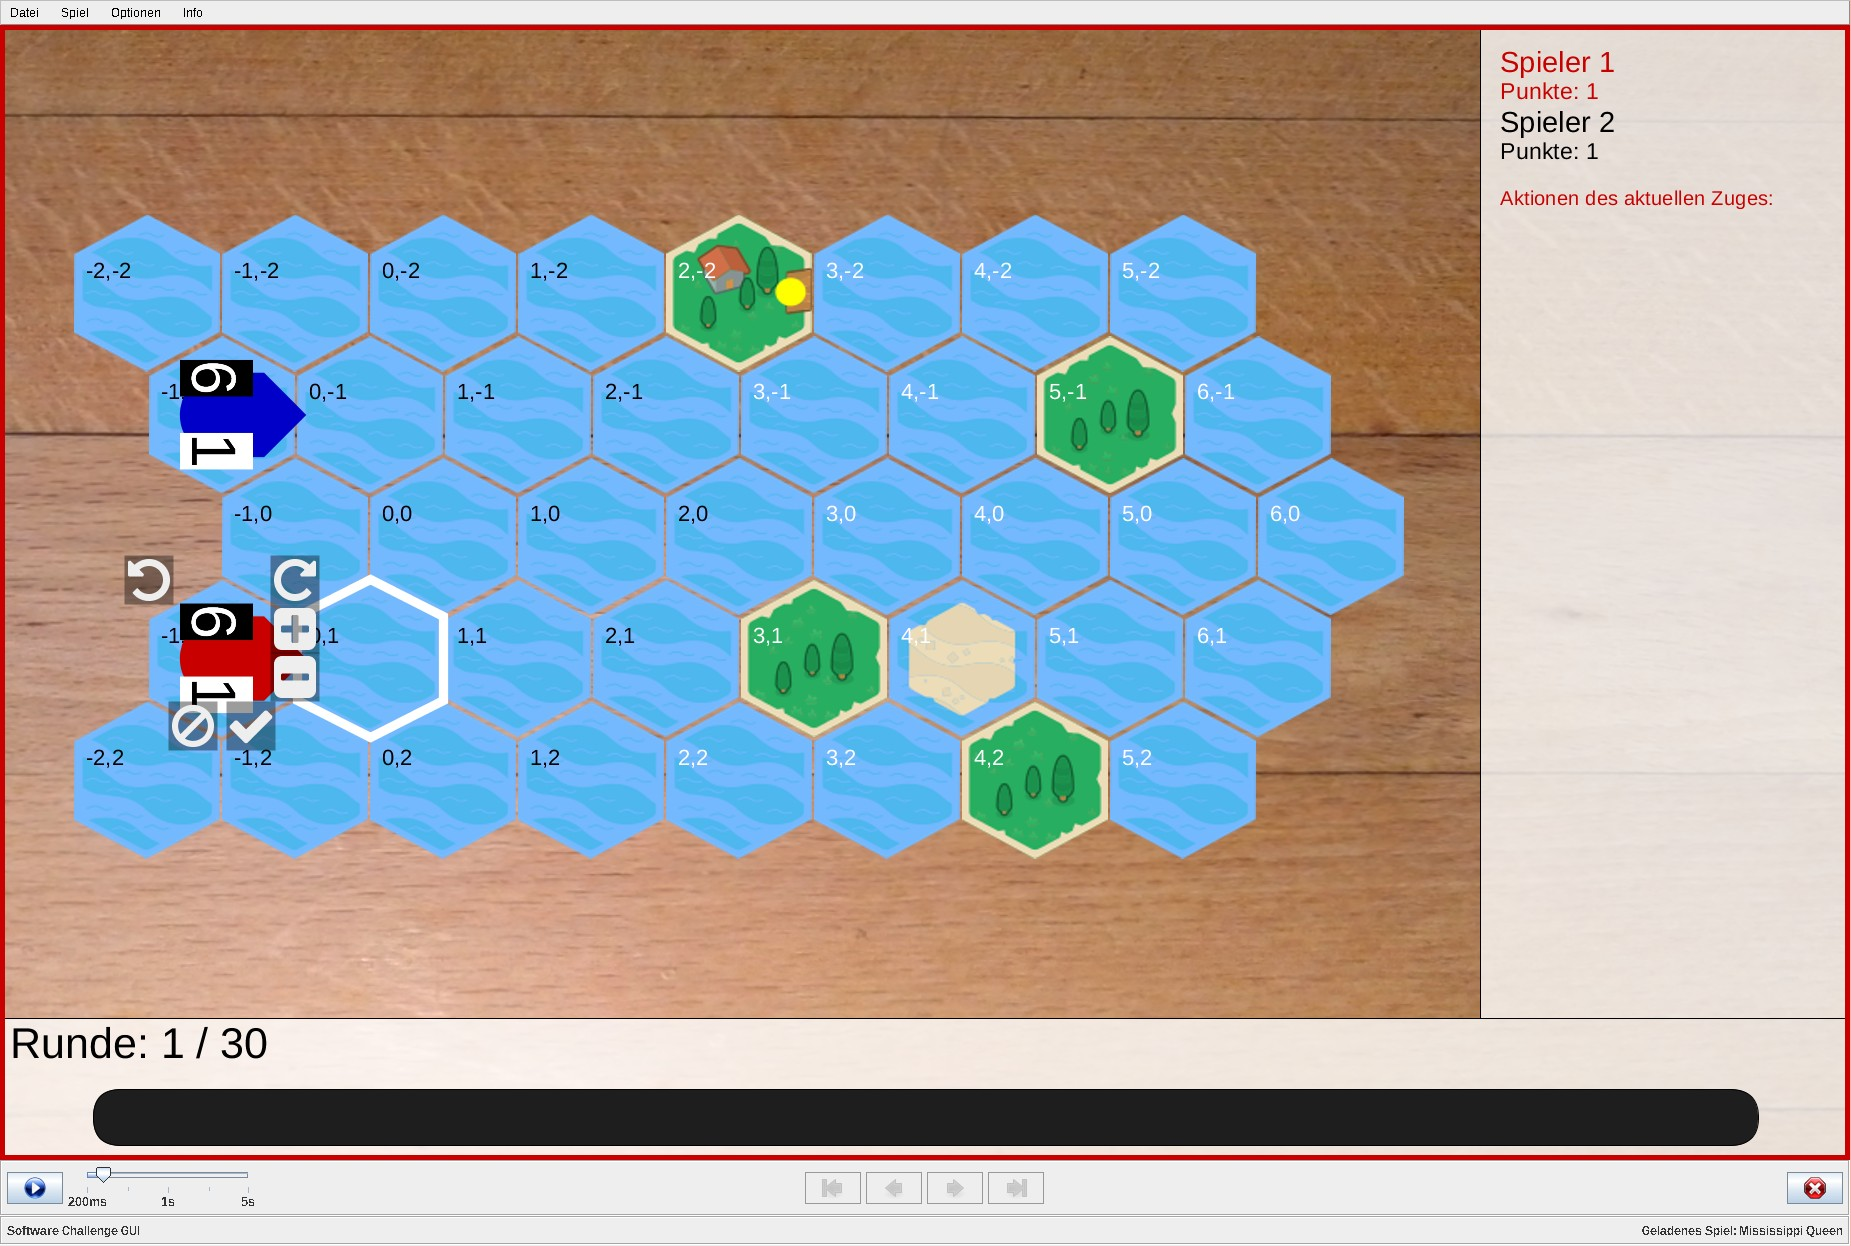
\includegraphics[width=\textwidth]{bilder/spielfeld-anfang.jpg}

Ein mögliches Spielbrett zu Beginn des Spiels sieht man oben. Ein Spielbrett
nachdem das Spiel schon etwas weiter fortgeschritten ist, sieht man auf der
Titelseite dieser Anleitung. Das gesamte Spielbrett besteht aus \Tiles/
Spielsegmenten mit jeweils \FieldsPerTile/ Feldern. Die Segmente kann man durch
die Farbe der Koordinaten auf den Feldern erkennen: Die Segmente haben
abwechselnd schwarze und weiße Koordinaten auf den Feldern. Am Anfang ist nur
das Startsegment und ein darauf folgendes Segment aufgedeckt. Diese beiden
Segmente sind immer gerade ausgerichtet, bilden also keinen Knick in eine
Richtung. Sobald ein Dampfer auf das zuletzt aufgedeckte Segment fährt, wird ein
neues dahinter aufgedeckt und zwar zufällig nach links, nach rechts oder mittig.
Dies geschieht solange, bis alle \Tiles/ Segmente aufgedeckt sind. Das letzte
Segment ist das Zielsegment (siehe Abbildung unter Spielende, Abschnitt
\ref{sec:spielende}). Segmente die schon von allen Spielern betreten und wieder
verlassen wurden, werden vom Spielplan entfernt, auch wenn sich darauf noch
Inseln mit Passagieren befinden.

Die Spielsegmente bestehen aus verschiedene Arten von Hexagon-Feldern, die
zufällig verteilt sind. Neben Wasserfeldern, Inseln, Sandbänken und Baumstämmen
gibt es pro Spiel insgesamt \Passagiere/ Passagierfelder.

Jeder Dampfer beginnt das Spiel mit einer Geschwindigkeit von 1 und einem
Kohlevorrat von 6. Der Dampfer hat außerdem eine von sechs Bewegungsrichtungen,
die den Seiten des Hexagon-Feldes entsprechen, aus denen die Segmente aufgebaut
sind. Die Geschwindigkeit eines Dampfers bestimmt, wie viele Bewegungspunkte er
in einer Runde zur Verfügung hat. Den Kohlevorrat kann man nutzen, um besondere
Aktionen durchzuführen und die Bewegungsrichtung bestimmt, wohin der Dampfer
gerade fährt.

\subsection{\label{water}Das Wasserfeld}

\fieldGraphic{r}{wasser}

Das Wasserfeld kann ganz normal befahren werden. Auf ein zum Spieler in der
aktuellen Bewegungsrichtung benachbartes Wasserfeld ziehen, kostet einen
Bewegungspunkt.

\paragraph{}

\subsection{\label{island}Die Insel}

\fieldGraphic{r}{insel}

Die Insel kann nicht überquert werden. Fährt ein Dampfer auf eine Insel (z.B.
weil er nicht rechtzeitig bremsen kann), hat er das Spiel verloren.

\paragraph{}

\subsection{\label{passenger}Das Passagierfeld mit Anleger in verschiedene Richtungen}

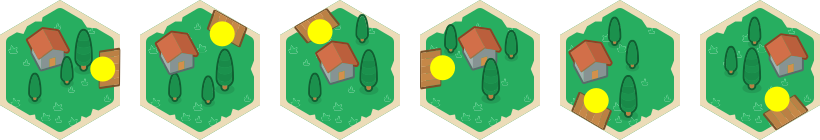
\includegraphics[width=\textwidth]{bilder/passagier}

Auf dem Passagierfeld mit Anleger wartet ein Passagier, der am Anleger abgeholt
werden kann. Um den Passagier abzuholen, muss der Dampfer mit Geschwindigkeit 1
am Anleger ankommen. Es verwandelt sich in ein normales Inselfeld, sobald der
Passagier abgeholt wurde (siehe Insel, \ref{island}).

Ein Dampfer, der so abgedrängt wird, dass er auf einem Feld mit Anleger landet,
kann einen Passagier aufnehmen, sofern er Geschwindigkeit 1 besitzt.


\subsection{\label{sandbank}Die Sandbank}

\fieldGraphic{r}{sandbank}

Eine Sandbank stoppt einen Dampfer, sollte er darauf fahren. Das heißt, wenn ein
Spieler auf eine Sandbank fährt, beendet dies seinen Zug und setzt seine
Geschwindigkeit auf 1. Die Sandbank kann im nächsten Zug nur rückwärts oder
vorwärts in der Bewegungsrichtung, mit der sie befahren wurde, wieder verlassen
werden. Verlässt man es rückwärts, kostet dies zusätzlich eine Kohleeinheit. Auf
einer Sandbank kann nicht gedreht oder Beschleunigt werden und ein Dampfer, der
sich darauf befindet, kann nicht abgedrängt werden.

\paragraph{}

\subsection{Das Baumstammfeld}

\fieldGraphic{r}{baumstaemme}

Das Ziehen in ein Baumstammfeld kostet zwei Bewegungspunkte statt einem.
Außerdem wird die Geschwindigkeit eines Schiffes, welches ein Baumstammfeld
durchquert nach dem Zug um 1 verringert. Sind nicht genug Bewegungspunkte
vorhanden, kann es nicht überquert werden. Das Abdrängen in ein Baumstammfeld
kostet einen zusätzlichen Bewegungspunkt.

\paragraph{}

\subsection{\label{goal}Das Zielfeld}

\fieldGraphic{r}{ziel}

Ein Zielfeld ist ein Feld, das erreicht werden kann, um das Spiel zu gewinnen.
Ein Zielfeld muss mit Geschwindigkeit 1 befahren werden und es müssen sich zwei
Passagiere an Bord befinden, damit der Dampfer das Spiel gewinnt. Sind diese
Bedingungen nicht erfüllt, kann ein Zielfeld wie ein Wasserfeld befahren werden.

Landet ein Dampfer durch abdrängen auf einem Zielfeld, reicht dies nicht zum
Gewinnen des Spiels, selbst wenn der abgedrängte Dampfer zwei Passagiere an Bord
hat und Geschwindigkeit 1 besitzt.

\paragraph{}

\section{Spielablauf}

Beide Spieler starten mit Geschwindigkeit 1 und 6 Kohleeinheiten und ziehen dann
jeweils einmal pro Runde. In der ersten Runde beginnt der rote Spieler. In allen
weiteren Runden wird der beginnende Spieler wie folgt ermittelt:

Es beginnt der Spieler

\begin{itemize}
\item dessen Dampfer sich am dichtesten am Ziel befindet (höchstes Segment oder bei gleichem Segment höchste Reihe, siehe Abbildung unter Abschnitt \ref{sec:spielende}).
\item Sollten beide Dampfer gleich dicht am Ziel sein, beginnt der Dampfer mit der höheren Geschwindigkeit.
\item Sollten beide Dampfer gleich schnell sein, beginnt der Dampfer mit dem höheren Kohlevorrat.
\item Sollten beide Dampfer gleich viel Kohle besitzen, beginnt der Dampfer, der am weitesten rechts steht (höchste X-Koordinate).
\item Sollten beide Dampfer gleich weit rechts stehen, beginnt der Dampfer, der am weitesten unten steht (höchste Y-Koordinate).
\end{itemize}

\section{Der Zug}

Ein Zug besteht aus einer oder mehreren Aktionen. In einem Zug
müssen (falls der Zug nicht auf einer Sandbank endet) durch die Aktionen
insgesamt alle Bewegungspunkte (bestimmt durch die Geschwindigkeit des Schiffes)
verbraucht werden. Die verschiedenen Aktionen sind:


\subsection{\label{acceleration}Beschleunigungsaktion}

Eine Beschleunigung kann nur als erste Aktion eines Zuges ausgeführt werden. Die
Beschleunigung um eine Geschwindigkeitseinheit pro Zug ist frei, jede
Beschleunigung um mehr als 1 kostet für jeden weiteren Geschwindigkeitspunkt
eine Kohleeinheit. Möchte ein Spieler beispielsweise mit einer aktuellen
Geschwindigkeit von 2 auf Geschwindigkeit 4 beschleunigen, kostet dies eine
Kohleeinheit. Die maximale Geschwindigkeit ist 6, die niedrigste 1.

Auf gleiche Weise kann auch abgebremst, also die Geschwindigkeit verringert
werden. Dies wird der Einfachheit halber als Beschleunigungsaktion mit negativer
Beschleunigung behandelt.

\subsection{Erzeugung der Bewegungspunkte}

Bevor nun eine der folgenden Aktionen durchgeführt werden kann, bekommt der
Dampfer entsprechend seiner aktuellen Geschwindigkeit Bewegungspunkte. Diese
Bewegungspunkte müssen durch die folgenden Aktionen aufgebraucht werden, am Ende
des Zuges dürfen also keine Bewegungspunkte mehr vorhanden sein.

\subsection{\label{turn}Drehaktion}

Eine Drehaktion je Zug des Spielers um eine Einheit (also um 60\degree) ist
frei. Jede weitere Drehung erfordert eine Kohleeinheit (Ausnahme Abdrängen,
siehe \ref{push}). Auf Sandbänken kann nicht gedreht werden.


\subsection{\label{push}Abdrängaktion}

Endet eine Aktion auf einem Feld mit dem gegnerischen Dampfer, muss darauf eine
Abdrängaktion folgen. Ein Spieler kann den Gegner auf ein beliebig angrenzendes,
jedoch nicht direkt hinter dem Spieler liegendes, begehbares Feld abdrängen
(\label{passierbar}Wasserfelder, Sändbänke und Baumstammfelder gelten als
begehbar). Eine Abdrängaktion kostet einen Bewegungspunkt, zwei, falls auf ein
Baumstammfeld abgedrängt wird. Es darf nicht von einer Sandbank aus abgedrängt
werden. Der abgedrängte Spieler bekommt eine zusätzliche freie Drehung für
seinen nächsten Zug. Wurde der Spieler auf eine Sandbank abgedrängt, entfällt
diese freie Drehung und die Geschwindigkeit des abgedrängten Spielers wird auf 1
reduziert.

\subsection{\label{step}Bewegungsaktion}

Eine Bewegungsaktion erfolgt in die derzeitige Bewegungsrichtung des Schiffes.
Sie kann nur über und auf passierbare (siehe \ref{passierbar}) Felder erfolgen.
Sie darf niemals durch ein vom Gegner besetztes Feld oder eine Sandbank gehen,
darf jedoch auf dem Feld des Gegners oder einer Sandbank enden. Es ist weiterhin
nicht erlaubt, durch das gesamte, zuletzt aufgedeckte Segment in ein noch nicht
aufgedecktes Feld zu ziehen.

\subsection{Kombination von Aktionen}

Solange die Regeln der einzelnen Aktionsarten eingehalten werden, können mehrere
Aktionen innerhalb eines Zuges beliebig kombiniert werden.

\section{Spielende}\label{sec:spielende}

\begin{centering}
  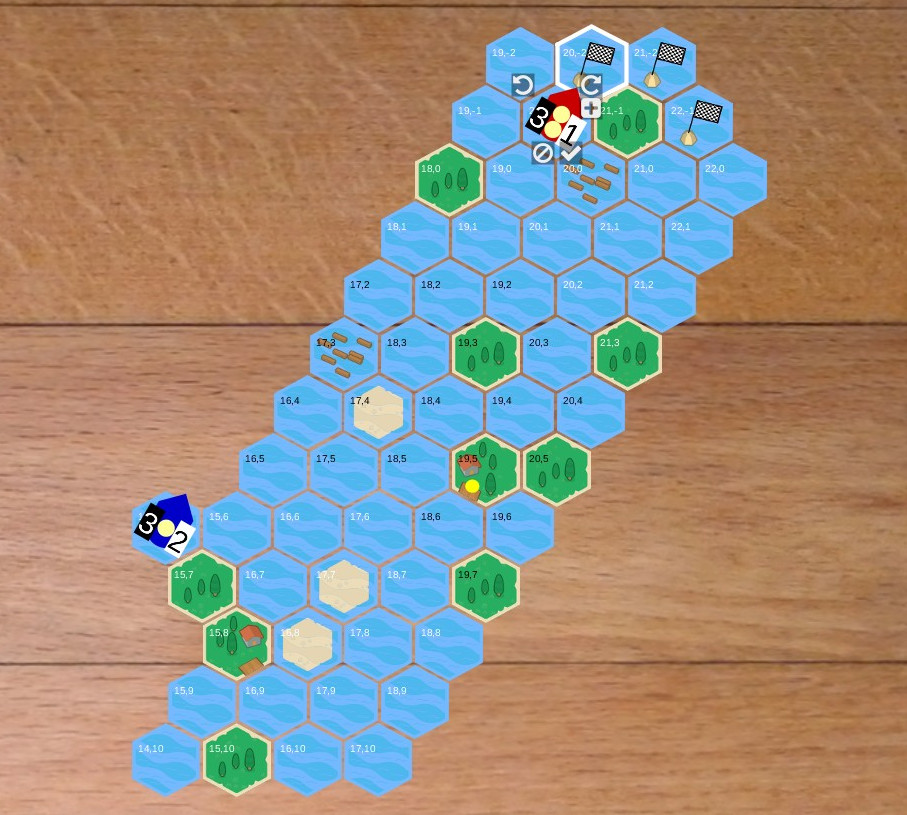
\includegraphics[width=\textwidth]{bilder/spielfeld-ziel.jpg}
\end{centering}

Das Spiel ist beendet, sobald

\begin{itemize}
\item ein Dampfer mit 2 Passagieren ein Zielfeld mit Geschwindigkeit 1 erreicht hat.
\item ein Spieler einen unültigen Zug macht.
\item am Ende einer Runde ein Dampfer mehr als 3 Spielsegmente zurückliegt.
  \item das Rundenlimit von 30 Runden erreicht ist.
\end{itemize}

Ein Spieler, der einen ungültigen Zug macht, erhält für das Spiel insgesamt 0
Punkte. In allen anderen Fällen berechnet sich der Punktestand eines jeden
Spielers folgendermaßen:

\begin{itemize}
  \item Jeder eingesammelte Passagier bringt 5 Punkte.
  \item Jedes überwundene Segment bringt 5 Punkte.
  \item Anhand der Position innerhalb eines Segments werden 0 bis 4 Punkte
    vergeben. Ein Segment ist aufgeteilt in 5 Reihen. Je weiter vorne man ist,
    desto mehr Punkte bekommt man (siehe Abbildung unten).
\end{itemize}

\begin{centering}
  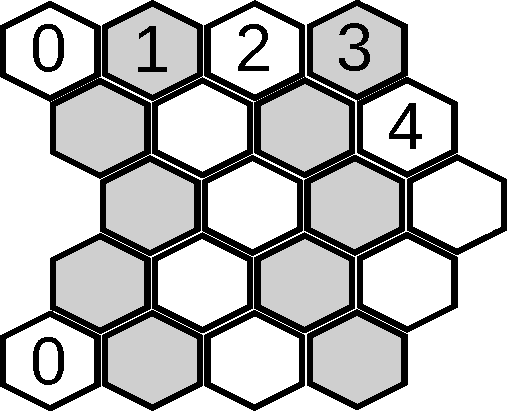
\includegraphics[width=0.6\textwidth]{bilder/segment-punkte.pdf}
\end{centering}

Bei Spielende gewinnt der Spieler mit den meisten Punkten. Sollten beide Spieler
gleich viele Punkte haben, gewinnt der Spieler, der mehr Passagiere eingesammelt
hat. Sollte auch diese Zahl gleich sein, endet das Spiel unentschieden.

\section{Die graphische Benutzeroberfläche für menschliche Spieler}

Über die grafische Benutzeroberfläche (auch GUI Server genannt) können zwei
menschliche Spieler gegeneinander oder ein menschlicher Spieler gegen einen
Computerspieler spielen (ausserdem kann man Spielaufzeichnungen abspielen und
Massentests von Computerspielern durchführen).

Die Bedienung des Spiels durch einen menschlichen Spieler wird im Folgenden
erklärt.

\subsection{Neues Spiel starten}

Nach dem Start der grafischen Oberfläche ist das Menü oben sowie die Statusleiste unten sichtbar. Der Rest des Fensters ist grau.

Um ein neues Spiel zu starten, wählt man im Menü unter ``Spiel'' ``Neues Spiel
erstellen'' aus.

{%
\centering%
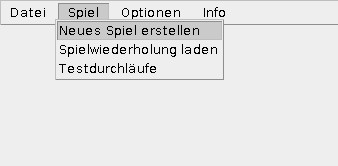
\includegraphics[width=0.4\textwidth]{bilder/neues-spiel-menu.jpg}
}

Nun erscheint ein Dialogfenster, in dem man die Einstellungen für das neue Spiel
bearbeiten kann. Zuerst kann man den Namen des ersten und zweiten Spielers
festlegen, indem man in das jeweilige Namensfeld klickt. Daneben befindet sich
die Auswahl, ob der jeweilige Spieler ein Mensch, ein Computerspieler oder ein
manuell gestarteter\footnote{Alle Computerspieler die nicht mit dem
  Software-Challenge Java SDK entwickelt wurden, müssen manuell gestartet
  werden.} Computerspieler sein soll. Wählt man hier ``Computerspieler''
erscheint ein Dateiauswahldialog, in dem man das JAR-Archiv mit dem
Computerspieler auswählen kann. In das letzte Feld können noch Parameter
eingegeben werden, die dem Computerspieler beim Start übergeben werden sollen
(dies ist nur bei Spielertyp ``Computerspieler'' relevant).

\begin{centering}
  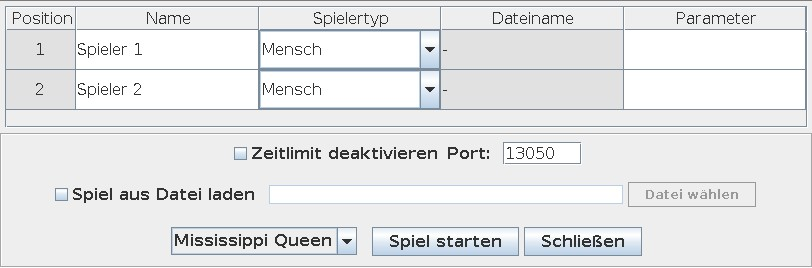
\includegraphics[width=\textwidth]{bilder/neues-spiel-dialog.jpg}
\end{centering}

Unter den Spielereinstellungen befinden sich noch weitere Einstellungen:

\begin{description}
\item [Zeitlimit deaktivieren] Wenn der Haken gesetzt wird, gilt für die Computerspieler nicht das Zeitlimit von 2 Sekunden pro Zug. Für menschliche Spieler gilt niemals ein Zeitlimit und diese Einstellung ist ohne Wirkung.
\item [Port] Die Portnummer, unter der der Server erreichbar ist. Für manuell gestartete Computerspieler wichtig, da diese sich über den hier angegebenen Port mit dem Server verbinden müssen, um am Spiel teilzunehmen.
\item [Spiel aus Datei laden] Ist diese Aktion aktiviert und eine Replay-Datei angegeben, wird statt eines zufällig generierten Spielbrettes das Spielbrett aus dem Replay für das neue Spiel verwendet.
\item [Auswahl des Spiels] Hier ist das aktuelle Spiel voreingestellt. Dies sollte nicht verändert werden.
\item [Spiel starten Knopf] Startet das Spiel mit den aktuellen Einstellungen.
\item [Schließen Knopf] Schließt den Dialog, ohne ein Spiel zu starten.
\end{description}

\subsection{Hauptbildschirm}

\begin{centering}
  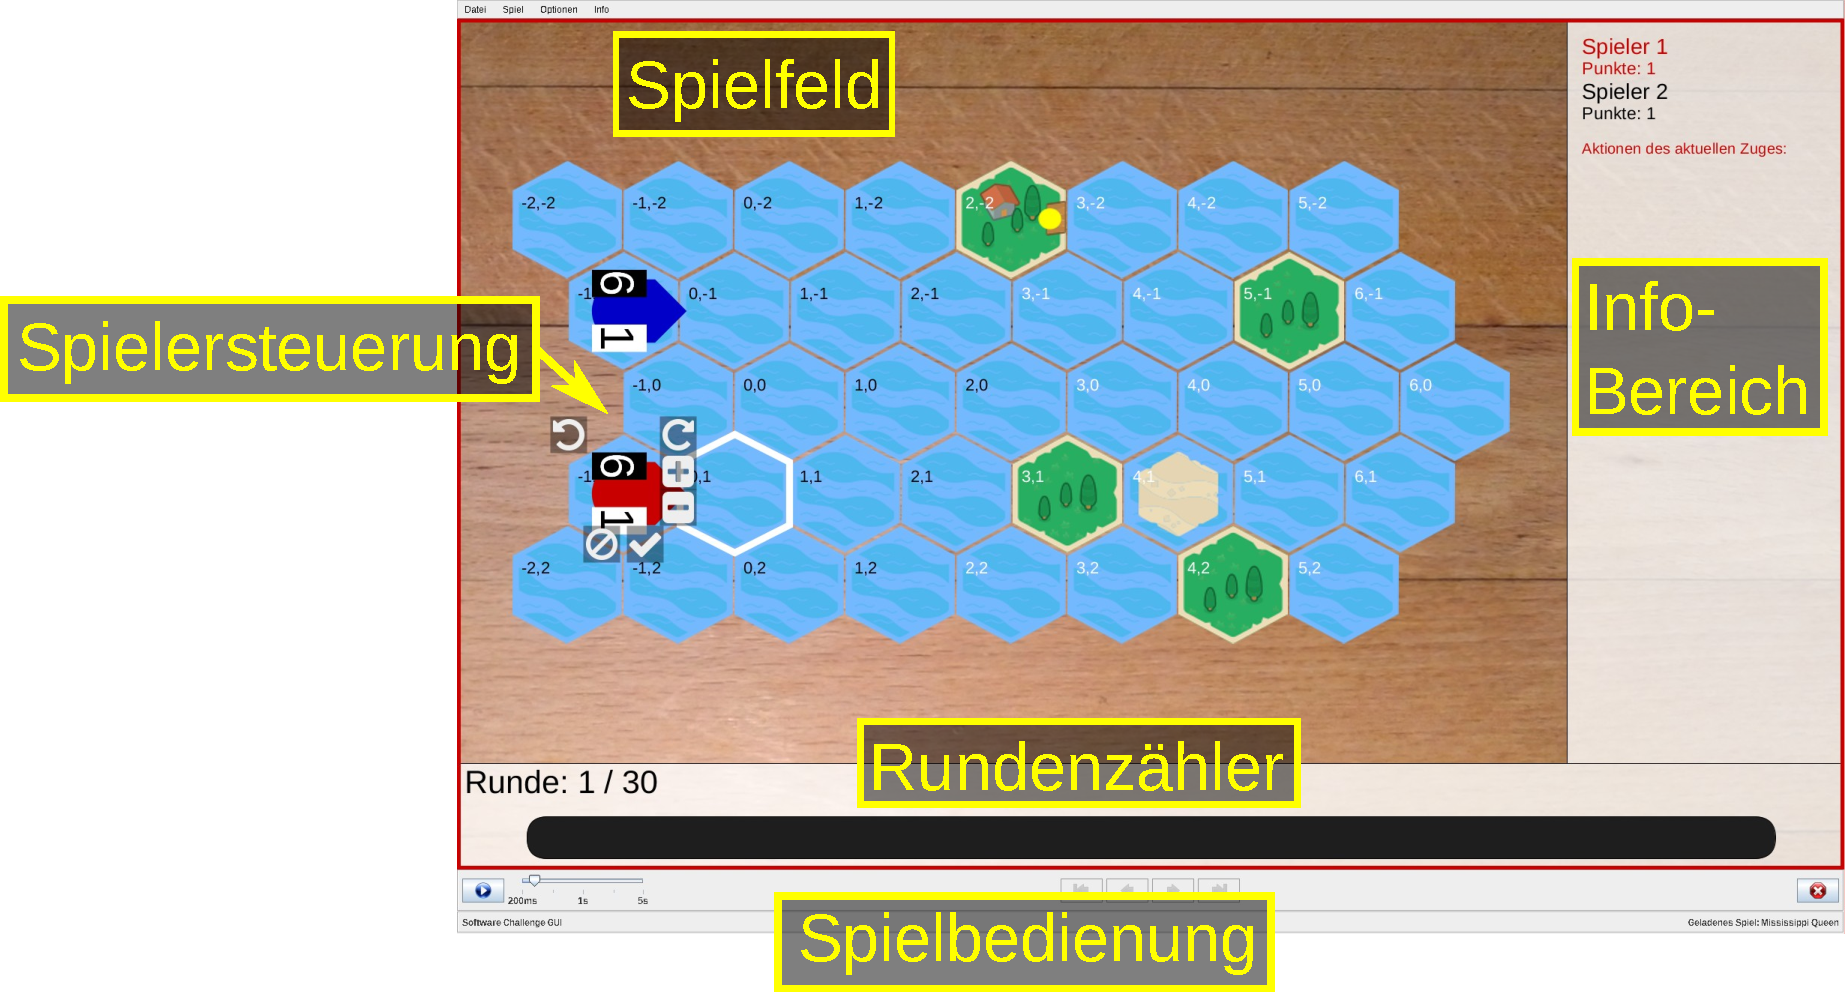
\includegraphics[width=\textwidth]{bilder/gui-elemente.pdf}
\end{centering}

In der obigen Abbildung sind die Grundelemente der grafischen Oberfläche des
Spiels dargestellt und beschriftet. Der Hauptbereich besteht aus der Darstellung
des Spielfeldes. In das Spielfeld eingebettet ist die Spielsteuerung, falls
gerade ein menschlicher Spieler am Zug ist. Rechts vom Hauptbereich befindet
sich ein Info-Bereich, in dem die Spielernamen, die bisher erreichten Punkte der
Spieler sowie die bisher gemachten Aktionen eines menschlichen Spielers im
aktuellen Zug textuell dargestellt werden. Unterhalb des Hauptbereichs und des
Info-Bereichs befindet sich der Rundenzähler, auf dem man die aktuelle Runde
ablesen kann. Darunter findet man die Bedienelemente zum kontrollieren des
Spielablaufes, die Spielbedienung.

\emph{Nach dem Starten eines neuen Spiels mit mindestens einem Computerspieler
  muss immer zuerst der ``Pause''-Knopf unten links angeklickt werden, sonst
  geht das Spiel nicht voran.}

\subsection{Dampfersteuerung}

Wenn ein menschlicher Spieler am Zug ist, kann er die Aktionen, die er in seinem
Zug durchführen will, über die Dampfersteuerung eingeben. Die Dampfersteuerung
besteht aus bis zu sechs Icons, die neben dem Dampfer des Spielers dargestellt
werden, sowie eventuell ein oder mehreren weiß umrandeten Hexagonal-Feldern.
Durch Klicken auf ein Dampfersteuerungselement wird die damit verbundene Aktion
ausgelöst. Die Aktionen sind im einzelnen:

\begin{table}[h!]
  \centering
  \begin{tabular}{ c m{0.7\linewidth} }
    Element & Beschreibung \\
    \hline
    \begin{minipage}{1cm}
      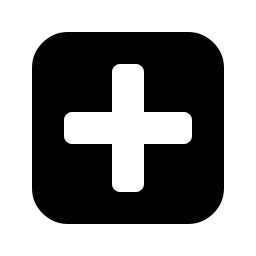
\includegraphics[width=\linewidth]{bilder/plus-square}
    \end{minipage}
    &
    Beschleunigung um 1. Wenn um mehr als 1 beschleunigt werden soll, entsprechend oft hintereinander anklicken. Beschleunigung ist nur als erste Aktion verfügbar.
    \\
    \begin{minipage}{1cm}
      
\includegraphics[width=\linewidth]{bilder/minus-square}
    \end{minipage}
    &
    Abbremsen um 1. Wenn um mehr als 1 abgebremst werden soll, entsprechend oft hintereinander anklicken. Abbremsen ist nur als erste Aktion verfügbar.
    \\
    \begin{minipage}{1cm}
      
\includegraphics[width=\linewidth]{bilder/rotate-left}
    \end{minipage}
    &
    Drehung um 60\degree nach links.
    \\
    \begin{minipage}{1cm}
      
\includegraphics[width=\linewidth]{bilder/rotate-right}
    \end{minipage}
    &
    Drehung um 60\degree nach rechts.
    \\
    \begin{minipage}{1cm}
      
\includegraphics[width=\linewidth]{bilder/okay}
    \end{minipage}
    &
    Zug ist vollständig. Falls der eingegebene Zug ungültig ist, erscheint
    eine Sicherheitsabfrage, ob man den Zug wirklich so durchführen möchte (was
    bei ungültigen Zügen zu einer Disqualifikation führt).
    \\
    \begin{minipage}{1cm}
      
\includegraphics[width=\linewidth]{bilder/cancel}
    \end{minipage}
    &
    Bisher eingegebene Aktionen löschen und mit der Eingabe von vorn beginnen.
    \\
    \begin{minipage}{1cm}
      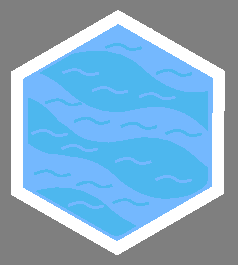
\includegraphics[width=\linewidth]{bilder/water-marked}
    \end{minipage}
    &
    Bewegung auf dieses Feld oder im Fall einer Abdrängaktion (siehe \ref{sec:push}): Abdrängen des Gegners auf dieses Feld.
  \end{tabular}
\end{table}

\subsection{Abdrängen}\label{sec:push}

\begin{centering}
  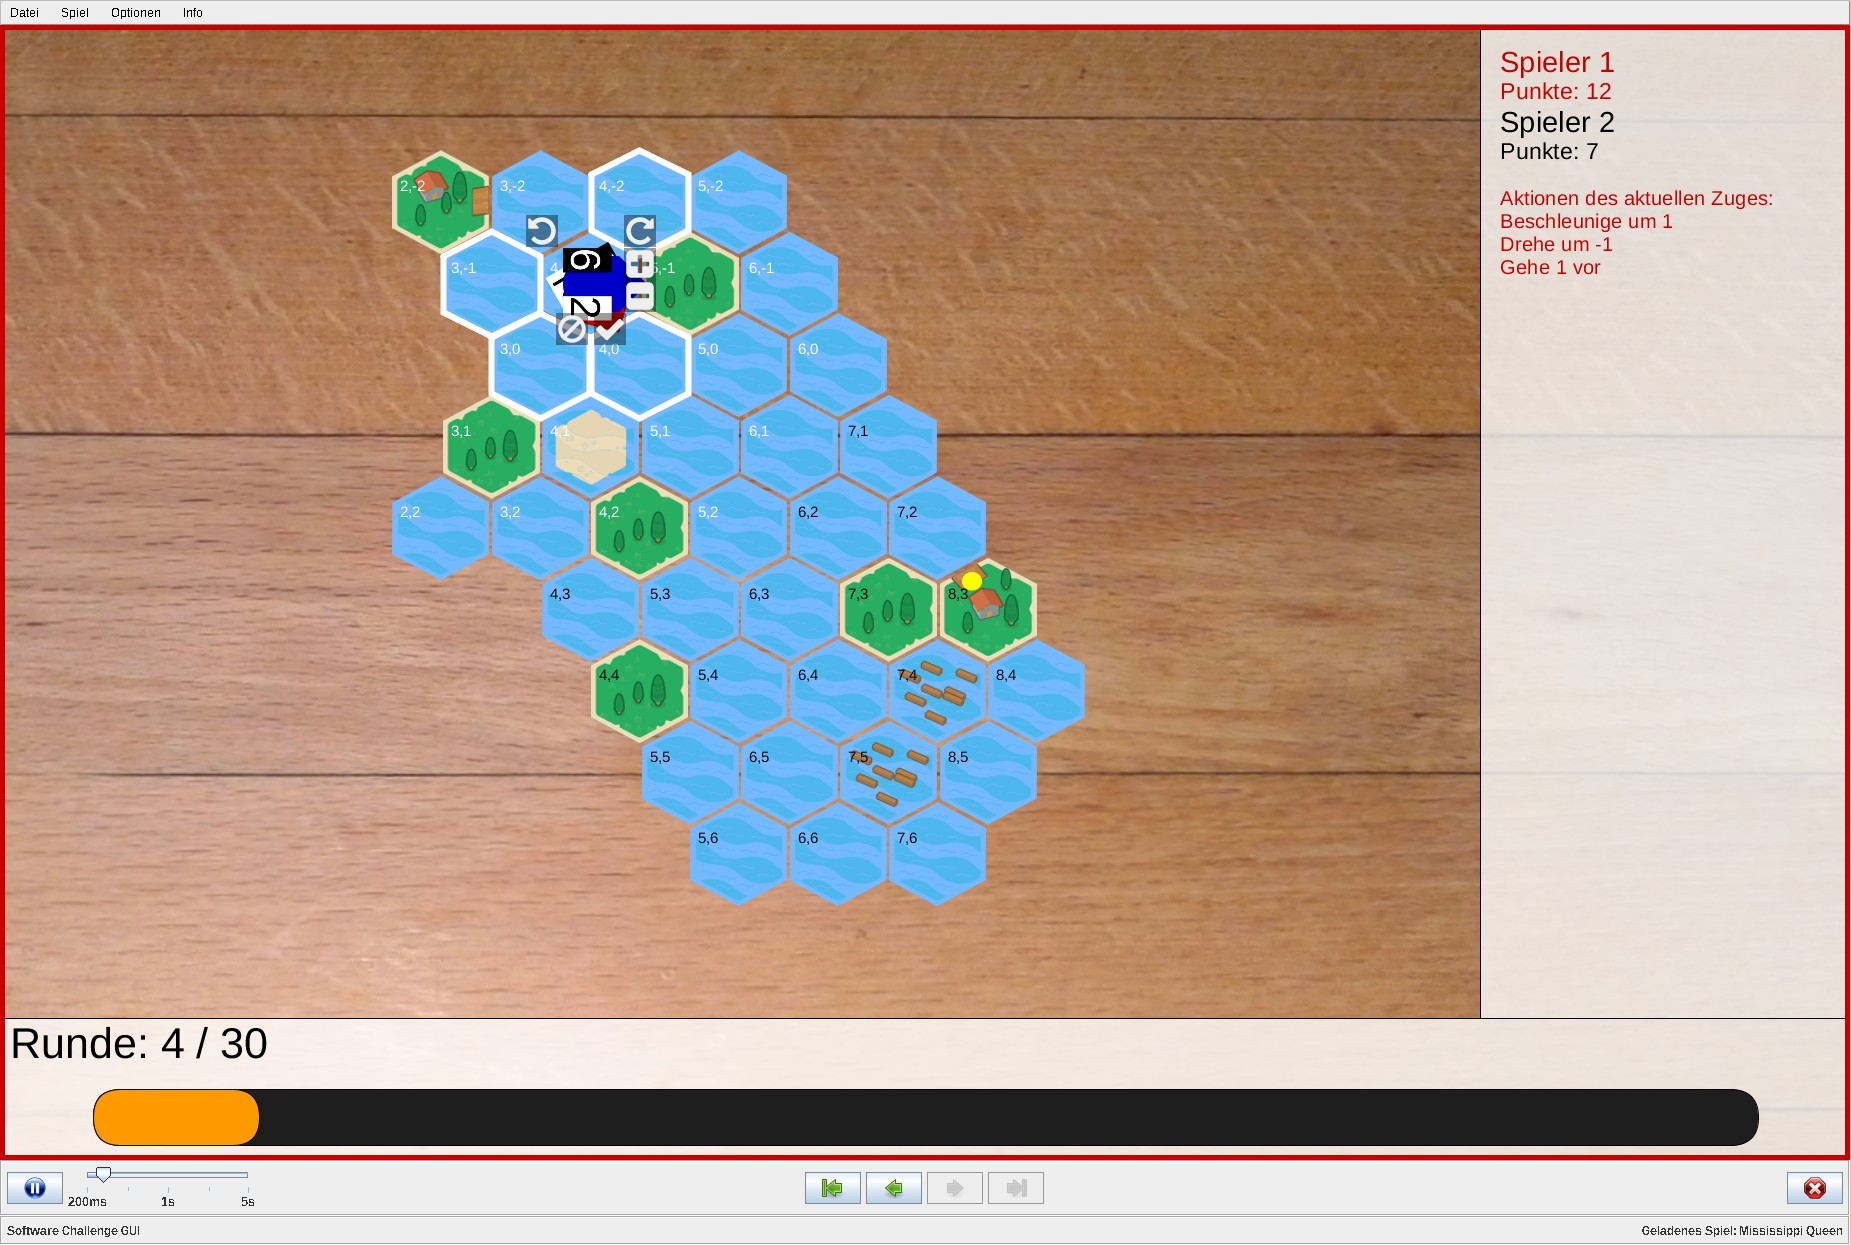
\includegraphics[width=\textwidth]{bilder/spielfeld-abdraengen.jpg}
\end{centering}

Sobald man durch eine Aktion auf das Feld des gegnerischen Dampfers kommt,
werden die Felder, auf die man den Gegner abdrängen kann, weiß umrandet. Durch
Klicken auf eines der weiß umrandeten Felder kann man den Gegner auf dieses Feld
abdrängen und die Abdräng-Aktion ist abgeschlossen.

\subsection{Passagiere aufnehmen}

Um Passagiere aufzunehmen, muss man wie unter \ref{passenger} beschrieben an
einen Anleger fahren. Beendet man dort seinen Zug mit Geschwindigkeit 1, wird
der Passagier automatisch aufgenommen.

\subsection{Spielbedienung}

Die Spielbedienung am unteren Rand des Fensters steuert das Abspielverhalten des
aktuellen Spiels. Diese kann verwendet werden, um bereits getätigte Züge
noch einmal anzusehen. Die einzelnen Elemente sind von links nach rechts:

\begin{description}
\item [Pause / Abspielen] Steht beim Start des Spiels auf ``Pause''. Damit das Spiel ablaufen kann, muss es auf ``Abspielen'' stehen.
\item [Geschwindigkeit-Schieberegler] Bestimmt die Zeit, die ein Zug beim Abspielen angezeigt wird.
\item [Zurück an den Anfang] Setzt das Spiel an den Anfang zurück.
\item [Schritt zurück] Geht eine Runde zurück.
\item [Schritt vor] Geht eine Runde vor.
\item [Vorspulen] Geht ans Ende des bisher gespielten Spieles.
\item [Spiel abbrechen] Beendet das Spiel.
\end{description}


\end{document}
